%******************************* DODATEK ***************************************
\appendix

\chapter{Urejanje dokumentov z orodjem LaTeX} \label{prilogaA}

\begin{description}
	\item[Korak 1] Avtor kreira tekstovno datoteko s končnico \emph{.tex}, ki vsebuje tekst in ukaze za oblikovanje teksta (oziroma se uporabi izvorna koda te predloge). Dober uvod v delo z ukazi LaTeX so spletna navodila \cite{oetiker1995not}. Za pisanje je lahko uporabljen katerikoli tekstovni urejevalnik. Priporočamo uporabo urejevalnikov WinEdt\footnote{Dostopno na: http://www.winedt.org} ali TeXstudio\footnote{Dostopno na: http://texstudio.sourceforge.net/}, ki sta namenski orodji z integriranimi ikonami za posamezne korake. Urejevalnika vsebujeta tudi slovar slovenskih besed\footnote{Dostopno na: http://www.winedt.org/Dict} za sprotno preverjanje in deljenje besed. Na spletu so na voljo tudi hitri priročniki z LaTeX ukazi\footnote{Primer dostopen na: https://en.wikibooks.org/wiki/Category:Book:LaTeX} in spletni urejevalniki\footnote{Primer dostopen na: https://overleaf.com}.
	\item[Korak 2] Prevajanje izvorne datoteke s prevajalnikom MiKTeX. Možnost direktnega prevajanja v PDF dokument (ikona LaTeX) pri prvem prevajanju ustvari tudi listo citatov in sklicevanj (datoteka \emph{.aux}).
	\begin{description}
		\item[Korak 2.1]\footnote{Potrebno samo pri navajanju virov s pomočjo orodja BibTeX} Zagon BibTeX prevajanja (ikona \emph{Bib}), ki na osnovi \emph{.aux} datoteke in podatkov iz baze referenc, ustvari oblikovan spisek referenc (datoteka \emph{.bbl}) glede na izbran stil citiranja (datoteka \emph{.bst}).
		\item[Korak 2.2]\footnote{Potrebno samo pri navajanju virov s pomočjo orodja BibTeX} Ponovno prevajanje s prevajalnikom MiKTeX, ki v glavni dokument vključi oblikovane reference iz datoteke \emph{.bbl}.
	\end{description}
	\item[Korak 3] Ponovno prevajanje s prevajalnikom MiKTeX, ki poveže spisek referenc z navedki v tekstu.
	\item[Korak 4a] Pretvorba oblikovanega dokumenta v format PostScript in nato izvoz v obliki PDF dokumenta:
	\begin{itemize}[noitemsep]
		\item ikona DVI-PS - pretvorba v datoteko \emph{.ps}
		\item Ogled PostScript datoteke s programom GhostView
		\item Pretvorba v PDF dokument: GhostView: File/Convert/pdfwrite, pri čimer je potrebno izbrati parametre za format PDF/A glede na spletna navodila\footnote{Dostopno na: http://svn.ghostscript.com/ghostscript/trunk/gs/doc/Ps2pdf.htm\#PDFA}.
	\end{itemize}
	V tem primeru morajo biti vse vključene slike v formatu PostScript. V tem načinu je možna tudi uporaba orodja PSfrag, ki omogoča zamenjavo tekstovnih elementov na originalni sliki s poljubnim tekstom ali enačbo.
	\item[Korak 4b] Pretvorba oblikovanega dokumenta neposredno v PDF format. Ikona PDFTexify. V tem primeru so vključene slike lahko le v formatu PDF, PNG, JPEG ali GIF. Format izhodnega dokumenta PDF/A, ki je zahtevan za oddajo v Repozitorij UL, je podprt v tej LaTeX predlogi\footnote{Dodatne informacije: https://www.mathstat.dal.ca/\textasciitilde selinger/pdfa/}. Alternativna možnost je generiranje standardne PDF datoteke in poznejša pretvorba v format PDF/A. To je možno narediti z enim izmed plačljivih programov (npr. Adobe Acrobat Professional, Nitro Pro) ali s spletnimi pretvorniki\footnote{Primer: https://docupub.com/pdfconvert/}. Pri slednjih je potrebno biti pozoren na morebitne vodne žige ali napake, ki lahko nastanejo pri pretvorbi.
\end{description}

\chapter{Vključevanje slik v LaTeX dokumente} \label{prilogaB}

Slike vključujemo z ukazom \texttt{\textbackslash includegraphics} v okolju \texttt{figure}. EPS slike morajo biti shranjene brez glave z bitno sliko za predogled. Dodaten paket PSfrag omogoča zamenjavo (prepis) napisov na vektorski sliki. Za uporabo je potrebna vključitev orodja z ukazom \texttt{\textbackslash usepackage\{psfrag\}}. Primer LaTeX kode za zamenjavo napisa $test$ na sliki z LaTeX simbolom $\epsilon \;[\mu]$ je:

\begin{footnotesize}
	\begin{verbatim}
		\begin{figure}[h]
			\centering
			\psfrag{test}[B1][B1][1][0]{$\epsilon \;[\mu]$}
			\includegraphics[width=0.75\columnwidth]{primer_vektorske_slike.eps}
			\caption{\label{oznaka_slike} Primer slike.}
		\end{figure}
	\end{verbatim}
\end{footnotesize}

Za vključitev vektorske slike je možno uporabiti tudi makro \textbackslash epsslika, ki je vključen v stil za predlogo. Prvi parameter v makroju \textbackslash epsslika je podnaslov, drugi pa je ime datoteke s sliko brez končnice (privzeta končnica je .eps) in hkrati tudi oznaka za sklicevanje na sliko. Pri uporabi tega ukaza morajo biti datoteke EPS v korenu delovnega direktorija. Za vključevanje slika ne sme imeti glave z bitno sliko za predogled. Pri stilu je za vključevanje slik potrebno izbrati ustrezno opcijo pdftex ali pctex, glede na to katero distribucijo LaTeX prevajalnika se uporablja za prevajanje. Primer je prikazan na sliki \ref{oblika_signalov_2}.

\begin{figure}[h]
	\centering
	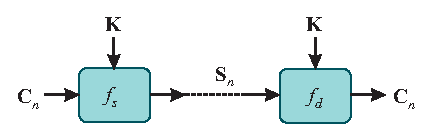
\includegraphics[width=0.75\columnwidth]{slike/vektorska_slika_2.eps}
	\caption{\label{oblika_signalov_2} Primer vektorske slike EPS.}
\end{figure}

Za vključevanje bitnih slik je v predlogi na voljo makro \textbackslash jpgslika. Prvi parameter v makroju \textbackslash jpgslika je podnaslov, drugi pa je ime datoteke s sliko (privzeta končnica je .jpg) in hkrati tudi oznaka za sklicevanje na sliko. Pri uporabi tega ukaza morajo biti slikovne datoteke v korenu delovnega direktorija. Slike so v tekst vključene v originalni velikosti.

Slika \ref{bitna_slika} predstavlja primer vključitve bitne slike JPG formata velikosti 9,4 x 7,6 cm.

\begin{figure}[h]
	\centering
	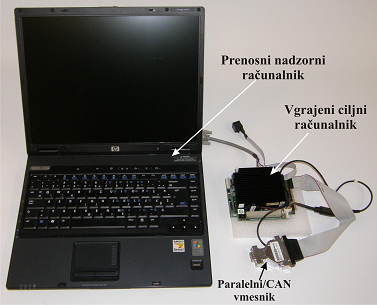
\includegraphics[width=9.4cm, height=7.6cm]{slike/bitna_slika.png}
	\caption{\label{bitna_slika} Primer vključitve bitne slike: sistem vodenja.}
\end{figure}

\chapter{Namestitev programskih orodij za urejanje LaTeX dokumentov} \label{prilogaC}

\section{Sistemi Windows}

\begin{description}
	\item[Korak 1] Namestitev paketa MiKTeX, ki je prevajalnik za dokumente, napisane v okolju LaTeX. Datoteke so dostopne na spletu: \url{http://miktex.org/}
	\item[Korak 2] Namestitev tekstovnega urejevalnika. Nekaj priporočenih:
	\begin{itemize}[noitemsep]
		\item TeXstudio (\url{http://texstudio.sourceforge.net/})
		\item Texmaker (\url{http://www.xm1math.net/texmaker/})
		\item Geany (\url{http://www.geany.org/})
		\item WinEdt (\url{http://www.winedt.com/})
	\end{itemize}
	\item[Korak 3] Namestitev ogledovalnika PostScript dokumentov:
	\begin{itemize}[noitemsep]
		\item modul GhostScript
		\item modul GhostView
	\end{itemize}
	Datoteke so dostopne na: \url{www.cs.wisc.edu/~ghost/}
\end{description}

Pri prvem prevajanju se lahko zgodi, da MiKTeX poskusi namestiti potrebne LaTeX knjižnice (pakete), kar mu je treba dovoliti, sicer predloga ne more delovati. Zaradi prenašanja in nameščanja prvo prevajanje lahko spodleti, kar je napaka paketa MiKTeX.

\section{Sistemi Linux}

Na sistemih Linux je potrebno za uporabo predloge namestiti naslednje pakete:

\begin{itemize}[noitemsep]
	\item \texttt{texlive-lang-european}
	\item \texttt{texlive-lang-greek}
	\item \texttt{texlive-latex-extra}
\end{itemize}

Imena paketov so povzeta po znani Linux distribuciji Ubuntu. V drugih distribucijah se enaki paketi lahko imenujejo tudi malo drugače. Za urejanje dokumentov se priporočajo naslednji tekstovni urejevalniki:

\begin{itemize}[noitemsep]
	\item TeXstudio (paket \texttt{texstudio})
	\item Texmaker (paket \texttt{texmaker})
	\item Geany (paket \texttt{geany})
\end{itemize}